The event yields shown in Table~\ref{tab:eventYieldCTagEx} have two types of uncertainties: statistical and systematics. For $N$ number of events, 
the absolute statistical uncertainty is $\sqrt{N}$. To calculate statistical uncertainties 
with the scale factors, applied in Sec~.\ref{s:secMCSF}, the histograms are filled with 
"Sumw2()" method. The systematics uncertainties arise due to improper calibration of the detector, 
the uncertainty in the efficiency of the reconstruction algorithm, uncertainty difference in 
theoretical prediction etc. The systematics uncertainties considered in this analysis are 
divided into two categories: experimental and theoretical uncertainties.

\subsection{Experimental Uncertainties}
\begin{itemize}
\item {\bf Luminosity}: The uncertainty in the integrated luminosity is 2.5\% for 2016 data taking~\cite{CMS-PAS-LUM-17-001}. 
\item {\bf Pileup reweighting}: The pileup weights as discussed in Sec.~\ref{s:pileup_reweighting}
    are calculated using minimum bias cross-section 69.2 mb. The uncertainty in the minimum 
    bias cross-section affects the pileup distribution of data of Figure~\ref{subfig:dataPileup}. 
    Hence the pileup weights of Figure~\ref{subfig:ratioPileup_all} is also affected. The 
    minimum bias cross-section is varied up and down by 4.7\% and corresponding pileup
    weights are applied to the MC events. The effect of pileup uncertainty on the \mjj
    shape is shown in Figure~\ref{subfig:sys_Pileup_wh_mu},~\ref{subfig:sys_Pileup_wh_ele} and
    Figure~\ref{subfig:sys_Pileup_ttbar_mu},~\ref{subfig:sys_Pileup_ttbar_ele} from charged Higgs
    and \ttjets sample, respectively.

\item {\bf Lepton trigger, tracking, identification and isolation}: 
    The lepton scale factors as discussed in Sec.~\ref{s:lepton_sf} are applied to the MC
    samples. A conservative 3\% uncertainty is considered on combined lepton scale factors
    for both channels. 

\item {\bf Jet energy, \MET correction}: The $\pt$ of jet in the MC are corrected using JES 
    and JER as discussed in Sec.~\ref{s:JEC}. The jet correction is propagated to correct 
    \MET. The \mjj shape of Sec.~\ref{s:secMassReco} are also affected by the 
    uncertainties in the JES, JER as shown in 
    Figures~\ref{subfig:sys_JES_wh_mu},~\ref{subfig:sys_JES_wh_ele},~\ref{subfig:sys_JER_wh_mu},
    ~\ref{subfig:sys_JER_wh_ele} for charged Higgs signal ($m_{H^+} = 120 \GeV$) and in 
     Figures~\ref{subfig:sys_JES_ttbar_mu},~\ref{subfig:sys_JES_ttbar_ele} 
    ~\ref{subfig:sys_JER_ttbar_mu},~\ref{subfig:sys_JER_ttbar_ele} for \ttjets 
    background in \mujets and \ejets channels. The uncertainties in the event 
    yield due to jet energy, \MET correction are shown in 
    Tables~\ref{tab:sysInc}, \ref{tab:sysCTagInc}, and \ref{tab:sysCTagEx} for different event categories.

    \item {\bf b/c-tagging uncertainty}: The b and c-jets are present within the same event. 
    The b/c tag scale factors (as described in Sec.~\ref{s:bTagSF} and Sec.~\ref{s:cTagSF}) 
    are correlated to each other as shown in Fig~\ref{fig:bcCorr}. 
    The correlated scale factors are varied up/down simultaneously. From Figure~\ref{fig:bcCorr}, 
    there are three nuisance parameters from various combination:
    \begin{figure}
    \begin{center}
    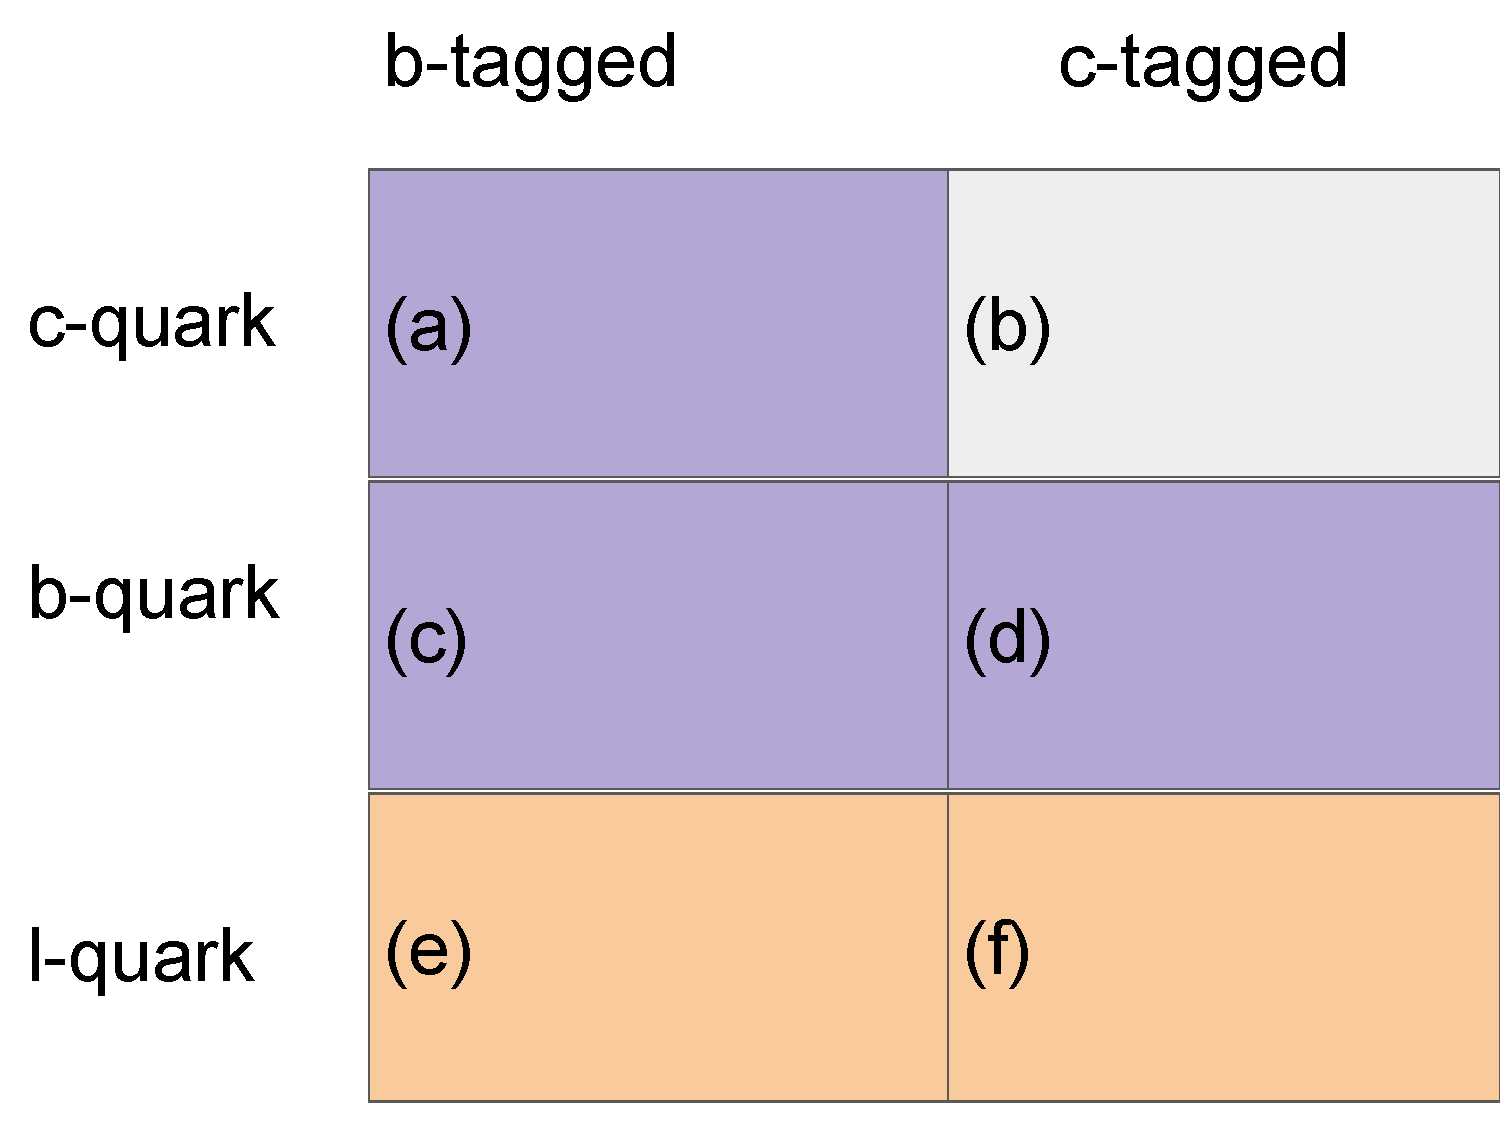
\includegraphics[width=0.50\textwidth]{Image/bcCorrelation.pdf}
    \caption{Correlation of b/c-tag scale factors. The region (a): c-quark tagged as b-jet, 
        (b): c-quark tagged as c-jet, (c): b-quark tagged as b-jet, (d): b-quark tagged as c-jet, 
        (e): light-quark tagged as b-jet, (f): light-quark tagged as c-jet.}
    \label{fig:bcCorr}
    \end{center}
    \end{figure}
    \begin{itemize}
    \item \verb|CMS_eff_bcInc3| (correlating (a), (c), (d))
    \item \verb|CMS_eff_bcInc2| (correlating (e), (f))
    \item \verb|CMS_eff_bcInc1| (from (b))
    \end{itemize}
    After $\geq$ 1 c-jet selection, the effect of b/c-tagging systematics on the shape of \mjj distribution are shown in    
    Figures~\ref{subfig:sys_bcTag1_wh_mu},~\ref{subfig:sys_bcTag2_wh_mu},~\ref{subfig:sys_bcTag3_wh_mu},
    and ~\ref{subfig:sys_bcTag1_wh_ele},~\ref{subfig:sys_bcTag2_wh_ele},~\ref{subfig:sys_bcTag3_wh_ele}
    for charged Higgs signal ($m_{H^+} = 120 \GeV$) and in
    Figures~\ref{subfig:sys_bcTag1_ttbar_mu},~\ref{subfig:sys_bcTag2_ttbar_mu},~\ref{subfig:sys_bcTag3_ttbar_mu},
    and
    ~\ref{subfig:sys_bcTag1_ttbar_ele},~\ref{subfig:sys_bcTag2_ttbar_ele}~,\ref{subfig:sys_bcTag3_ttbar_ele}
    for \ttjets background in \mujets and \ejets channels.
    The uncertainties on the event yield are shown in 
    Tables~\ref{tab:sysInc}, \ref{tab:sysCTagInc}, and \ref{tab:sysCTagEx} for different event categories.                                 

\item {\bf QCD data-driven uncertainty}: The relative isolation of muon(electron) 
    are conservatively shifted to 0.17 (0.11) and the corresponding change in the 
    QCD yield is determined. The percentage change in the yield is considered as 
    systematic uncertainty in the QCD estimation.
\item {\bf Bin-by-bin uncertainty}: In some of the bins of \mjj distributions, the
    statistics are small hence statistical uncertainty is large. In each bin of
    summed \mjj from all backgrounds, one shape nuisance is considered using 
    "autoMCStats" method (* autoMCStats 0 1) of Higgs combine tool.
\end{itemize}

\subsection{Theoretical Uncertainties}
\begin{itemize}
\item {\bf Normalization}: The MC events are normalised with the scale factor of 
    Eq.~\ref{eq:lumiSF}. The cross-section in Eq.~\ref{eq:lumiSF} have uncertainties. 
    The normalization uncertainties for MC samples are shown in 
    Tables~\ref{tab:sysInc}, \ref{tab:sysCTagInc}, and \ref{tab:sysCTagEx} for different event categories.
\item {\bf Top-quark \pt re-weighting}: The \PQt quark \pt weights are 
    determined from following equation
    \begin{equation}
    w_{top}=\sqrt{SF(t)\times SF(\bar{t})}, \quad{\rm where}\quad SF\equiv\exp(0.09494 - 0.00084\times\pt).
    \label{eq:top_wt}
    \end{equation}
    The values in the exponent are determined by fitting the inverse 
    of the ratio plot of Figure 3 of TOP-17-014 using the function
    $\exp(a + bx)$, where a and b are the parameters of the fit and x is
    the \pt of parton level \PQt quark. The corresponding $\chi^2$
    per number of  degree of freedom of the fit is 0.000985. 
    
    The parton level $\pt$ of $t$ and $\bar{t}$ quark is used to 
    calculate $SF$. The PDG code "6" and isLastCopy() is used to 
    identify the \PQt quark at parton level. The $w_{top}$ is taken to be 
    1 for "down" and $w_{top}^2$ for "up" systematic as recommended by 
    TOP-PAG~\cite{TopPtReweight}. The re-weighting is applied only 
    on \ttjets and charged Higgs samples shown in 
    Table~\ref{tab:mcSample}. The effect of top-pt re-weighting 
    uncertainties on the \mjj is shown in Figures~\ref{subfig:sys_topPt_wh_mu},
    ~\ref{subfig:sys_topPt_wh_ele}, for charged Higgs signal 
    ($m_{H^+} = 120 \GeV$) and in Figures~\ref{subfig:sys_topPt_ttbar_mu}, 
    ~\ref{subfig:sys_topPt_ttbar_ele} for \ttjets background in 
    \mujets and \ejets channels. 

    It is to be noted that the the analysis TOP-17-014 has dilepton in
    the final states whereas in this analysis (HIG-18-021) we have one
    lepton. A series of checks~\cite{ref:topPt} were performed to make 
    sure the SF are compatible with this analysis such as 
    \begin{itemize}
    \item 
    Kinematic selection of leptons and jets are very close between 
    the two analyses
    \item 
    The dilepton selection in TOP-17-014 is orthogonal to lepton+jets 
    selection of this analysis
    \item 
    The range of \pt of \PQt quark in the \ttbar MC in this analysis 
    is in the range of order of 500 \GeV as beyond this range the 
    extrapolation of weights are not reliable
    \item 
    The difference in the \pt spectrum of the \PQt quark between 
    nominal \ttbar (NLO PowHeg) and nominal signal (LO MadGraph) is 
    ~10\% and between reweighted \ttbar bkg (NLO PowHeg) and nominal 
    signal (LO MadGraph) is ~20\%. Because of the small difference, 
    the same SF is used for \ttbar and all signal samples.
    \end{itemize}

\item {\bf Top-quark mass}: The POWHEG \ttjets sample shown in Table~\ref{tab:mcSample} was 
    generated with $M_{t} =172.5$ \GeV. We used \ttjets sample with $M_{t} =171.5$ 
    \GeV and $M_{t} =173.5$ \GeV, as shown in Table~\ref{tab:mcSampleSys}, to observe the 
    effect of top-quark mass on the \mjj. The \mjj for different $M_t$ are shown  
    in Figures~\ref{subfig:sys_mass_ttbar_mu},~\ref{subfig:sys_mass_ttbar_ele}
    for \ttjets background in \mujets and \ejets channels. 

\item {\bf Parton shower matching}: In the POWHEG + PYTHIA generated samples, the 
    next-to-leading order (NLO) matrix element parton shower matching is varied by $h_{damp}$
    parameter. The \ttjets samples generated by varying $h_{damp}$ "up" and 
    "down", as shown in Table~\ref{tab:mcSampleSys} are used to see the effect of $h_{damp}$ 
    on the \mjj distribution as shown  
    in Figures~\ref{subfig:sys_matching_ttbar_mu},~\ref{subfig:sys_matching_ttbar_ele}
    for \ttjets background in \mujets and \ejets channels. 

\item {\bf Renormalization and factorisation scale}: To see the effect of renormalization and factorisation
    scale, the "up" and "down" \ttjets samples as shown in Table~\ref{tab:mcSampleSys}. The effect
    of these scales on the \mjj are shown 
    in Figures~\ref{subfig:sys_scale_ttbar_mu},~\ref{subfig:sys_scale_ttbar_ele}
    for \ttjets background in \mujets and \ejets channels. 
\end{itemize}
The QCD is estimated from data. Hence none of the systematics (except the QCD data-driven and 
normalization uncertainty) are considered on the QCD background. All the systematic
and statistical uncertainties are shown in Tables~\ref{tab:sysInc}, \ref{tab:sysCTagInc}, 
and \ref{tab:sysCTagEx} for different event categories.


